\subsection{{\bf Ablation Study (RQ4)}}
\label{empirical-rq3}

\subsubsection{Impact of Dual-Task Learning}
\label{sec:dual-task-result}


\begin{figure}[t]%[thbp]
\begin{center}
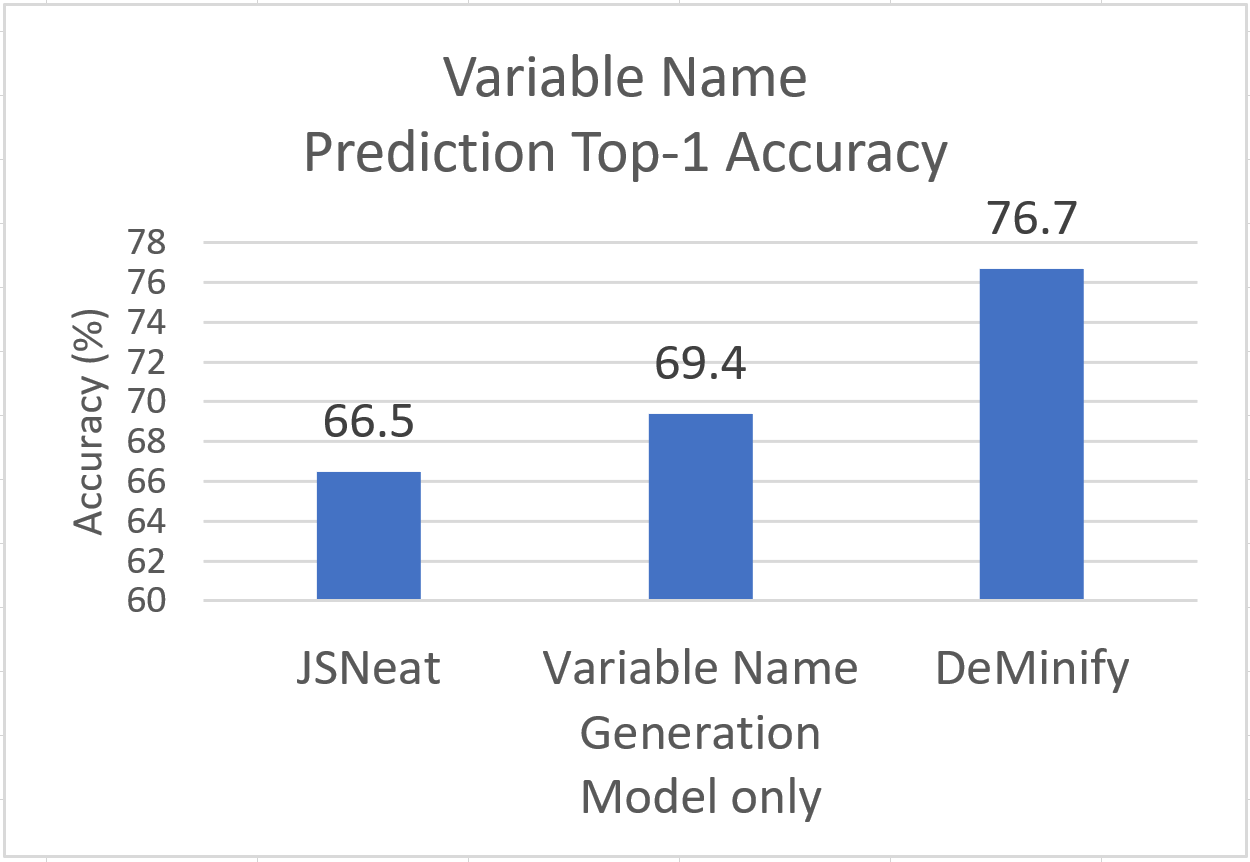
\includegraphics[width=2.5in]{figures/dual-task-result-11}
\vspace{-8pt}
\caption{RQ3. Impact of Dual-Task Learning on Variable Name Prediction}
\label{dual-task-result-1}
\end{center}
\end{figure}

\begin{figure}[t]%[thbp]
\begin{center}
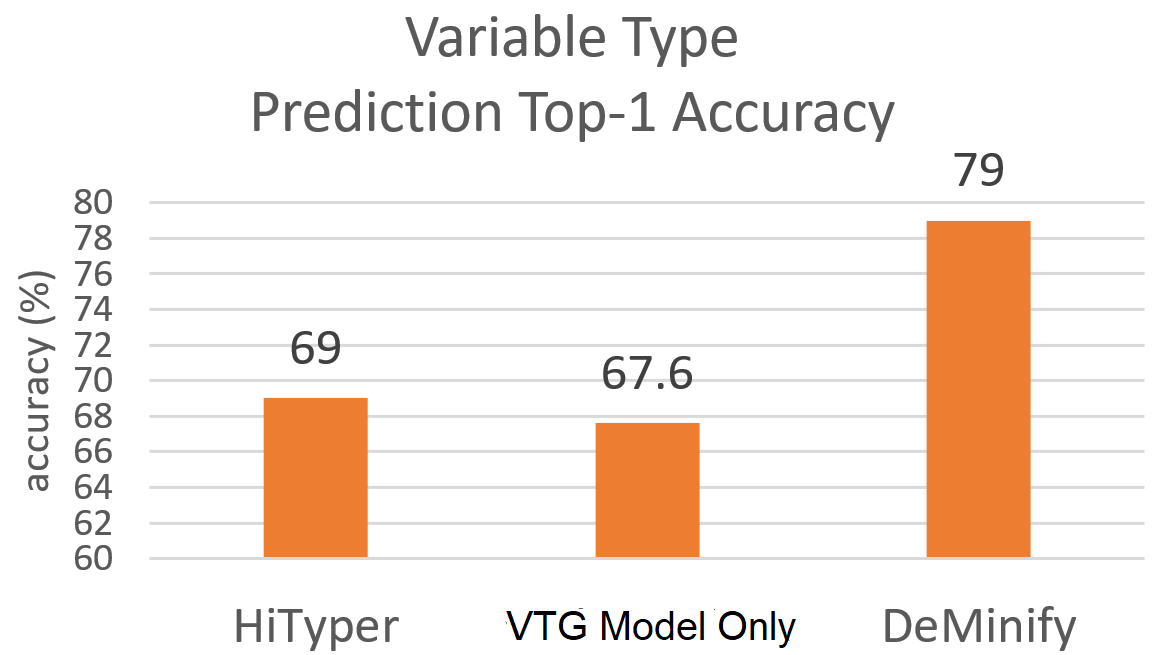
\includegraphics[width=2.5in]{figures/dual-task-result-22}
\vspace{-8pt}
\caption{RQ3. Impact of Dual-Task Learning on Type Prediction}
\label{dual-task-result-2}
\end{center}
\end{figure}

Figure~\ref{dual-task-result-1} shows the Top-1 accuracy in variable
name prediction when we removed the dual-task learning scheme and
measured only the accuracy of the variable name generation (VNG)
model.  As seen, without the impact from variable type generation
(VTG) via dual-task learning, VNG still performs better than the best
baseline, JSNeat (69.4\% versus 66.5\%). The drop in Top-1 accuracy
from {\tool} is 10.5\% (from 76.7\% downto 69.4\%). Similarly, as seen
in Figure~\ref{dual-task-result-2}, without the impact from VNG due to
the removal of the dual-task learning scheme, VTG performs slightly
worse than the best baseline HiTyper. The drop in Top-1 accuracy from
{\tool} is 14.4\%.  These results indicate the positive contribution to {\tool}
from our key ideas on the mutual impact of VNG and VTG via dual-task
learning.


\subsubsection{Impact of Different Types of Program Graphs}
\label{sec:graphs}

\begin{figure}[t]%[thbp]
\begin{center}
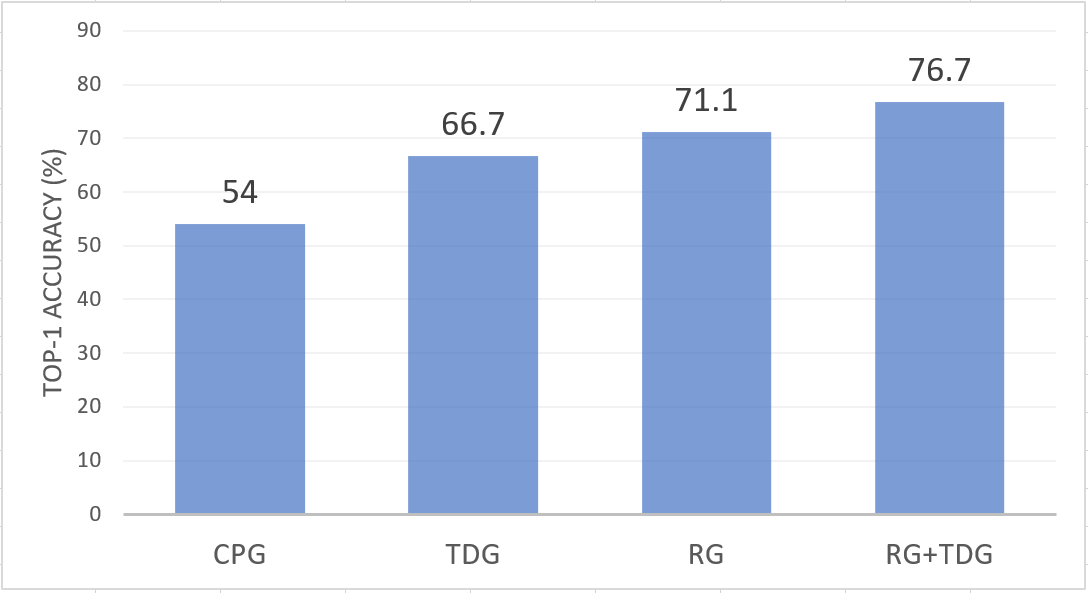
\includegraphics[width=2.3in]{figures/sensi-graphs-name-2}
\vspace{-8pt}
\caption{RQ4. Impact of Input Graphs on Name Prediction}
\label{graph-name-result}
{\bf CPG}: Code Property Graph, {\bf TDG}: Type Dependency Graph, {\bf RG}:Relation Graph. 
\end{center}
\end{figure}



As in any approach, code representation is
important and affects the performance. In this study, we
kept the same neural network architecture, however, changed different
input graphs extracted from source code. In addition to the graphs
used in {\tool} (Relation Graph (RG), Type Dependency Graph (TDG)), we
experimented with code property graph (CPG)~\cite{CPG-2014} since
it has been used in several machine learning approaches for
code~\cite{CPG-2014}. We did not experiment with program dependence
graph (PDG) because it works at the statement level, which does not
help with variable name prediction.

As seen in Figure~\ref{graph-name-result} and
Figure~\ref{graph-type-result}, for variable name prediction, RG helps
the model more than TDG and for variable type prediction, TDG helps
the model more than RG. This is expected because each of them is
designed toward capturing the key features for its problem. For the
dual tasks, the combined graph (RG+TDG) in {\tool} yields the highest
accuracies in both name prediction and type prediction. In contrast,
CPG capturing the dependencies among program elements are not
specifically designed for handling variable names and types, thus, did not
yield high accuracy as TDG, RG, and CG. An interesting observation is
that CPG, which contains lexical, syntax, and dependency information,
did not help the model as much as others. It seems that CPG contains
too much irrelevant information for variable name and type prediction.

\begin{figure}[t]%[thbp]
\begin{center}
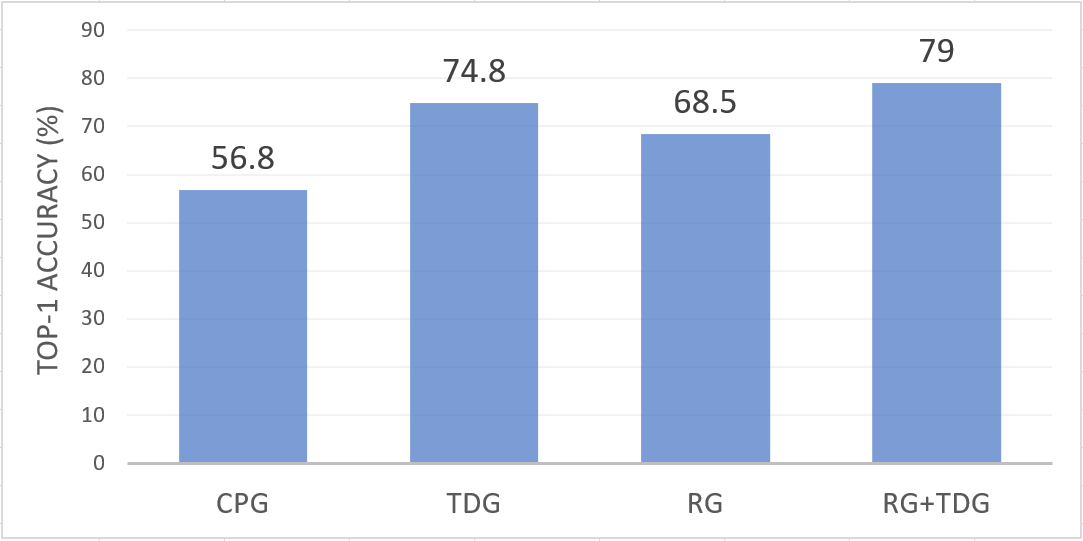
\includegraphics[width=2.3in]{figures/sensi-graphs-type-2}
\vspace{-8pt}
\caption{RQ4. Impact of Input Graphs on Type Prediction}
\label{graph-type-result}
{\bf CPG}: Code Property Graph, {\bf TDG}: Type Dependency Graph, {\bf RG}:Relation Graph.
\end{center}
\end{figure}

%1. Code property graph is complex but cannot represent the variable relationships and type changes clearly (EEGCN+GCNmf+CPG compared with EEGCN+GCNmf+RG on name prediction; EEGCN+GCNmf+CPG compared with EEGCN+GCNmf+TDG on type prediction)




\subsubsection{Impact of Graph Models}
\label{sec:models}

%\begin{figure}[thbp]
%\begin{center}
%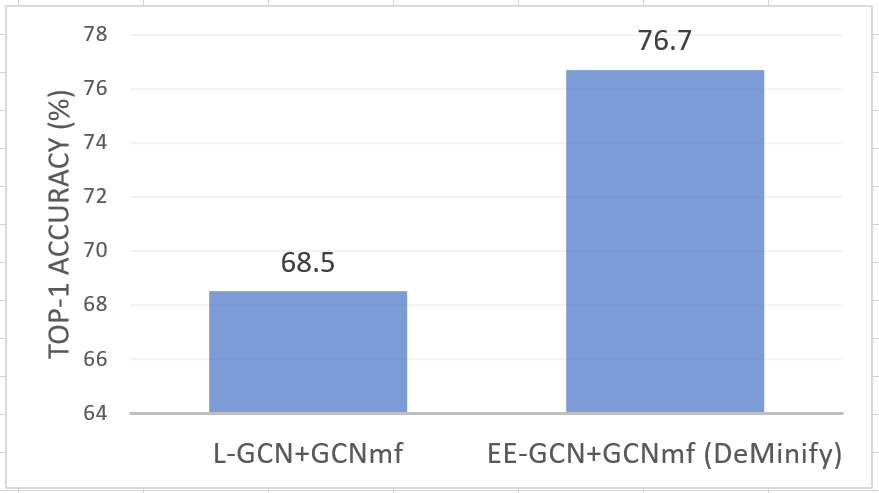
\includegraphics[width=2.6in]{figures/sensi-models-name}
%\vspace{-8pt}
%\caption{RQ3. Impact of Graph Model on Variable Name Prediction}
%\label{models-name-result}
%{\bf L-GCN}: Label Graph Convolutional Network, {\bf EE-GCN}: Edge-Enhanced Graph Convolutional Network, {\bf GCNmf}: Graph Convolutional Network - Missing Features
%\end{center}
%\end{figure}

%\begin{figure}[thbp]
%\begin{center}
%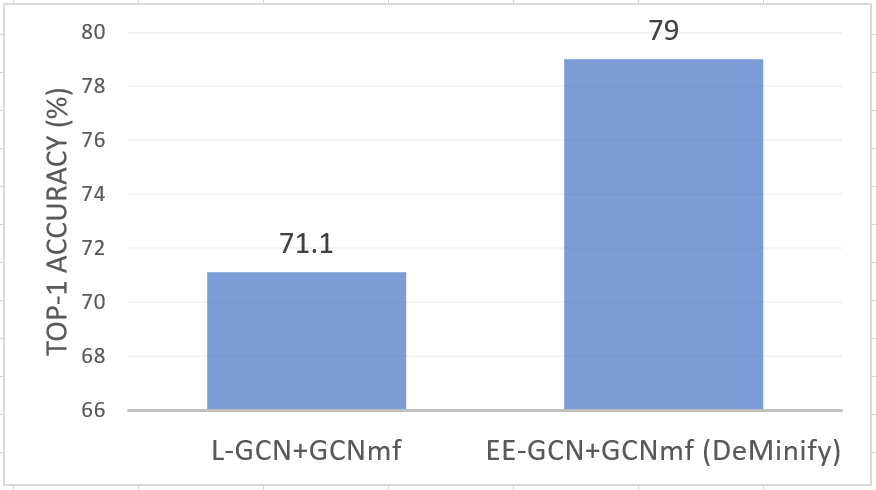
\includegraphics[width=2.6in]{figures/sensi-models-type}
%\vspace{-8pt}
%\caption{RQ3. Impact of Graph Model on Variable Type Prediction}
%\label{models-type-result}
%{\bf L-GCN}: Label Graph Convolutional Network, {\bf EE-GCN}: Edge-Enhanced Graph Convolutional Network, {\bf GCNmf}: Graph Convolutional Network - Missing Features
%\end{center}
%\end{figure}



Table~\ref{tab:sensi-graph} shows the accuracy of the variant model
as we replaced the graph neural network EE-GCN with the Label Graph
Convolutional Network (Label-GCN)~\cite{label-gcn}. We did not replace
GCNmf because it is the core component in our solution, which
formulates the name/type recovery as the prediction of missing
features. As seen, Edge-Enhanced GCN helps improve accuracy more than
Label-GCN. EE-GCN enables the modeling of different types of relations
because it handles different edge types in different channels, while
Label-GCN just integrates the edge information as simple labels.
This is crucial for our problem in which the type dependencies
and the variable relations are well captured.


\begin{table}[t]%[!ht]
  \centering
  \tabcolsep 2.5pt
    \begin{tabular}{|l|l|l|}
    \hline
        Accuracy (\%) & Name Prediction & Type Prediction\\ \hline
        Label-GCN+GCNmf & 68.5 & 71.1 \\ \hline
        EE-GCN+GCNmf (DeMinify) & 76.7 & 79 \\ \hline
    \end{tabular}
    {\bf Label-GCN}: Label Graph Convolutional Network, {\bf EE-GCN}: Edge-Enhanced Graph Convolutional Network, {\bf GCNmf}: Graph Convolutional Network - Missing Features
    \caption{Impact of EE-GCN on Top-1 Accuracy}
    \vspace{-10pt}
    \label{tab:sensi-graph}
\end{table}

%2. EEGCN is a more advanced model by representing the edge in $N$ channels instead of a simple label compared with label-GCN (EEGCN+GCNmf+RG compared with LGCN+GCNmf+RG on both two tables)


%\begin{table}[t]
%	\caption{RQ3. Sensitivity Analysis on Variable Name Prediction.}
%	\begin{center}
%		\small
%		\renewcommand{\arraystretch}{1} 
%		\begin{tabular}{p{2.5cm}<{\centering}|p{2cm}<{\centering}|p{2cm}<{\centering}}
%			\hline
%			                    & Local Variables & All Variables\\
%			\hline
%			LGCN+GCNmf+RG       & 0.69            & 0.77    \\
%			EEGCN+GCNmf+CPG     & 0.65            & 0.74    \\
%			EEGCN+GCNmf+RG      & 0.70            & 0.77    \\
%			EEGCN+GCNmf+TDG     & 0.66            & 0.75    \\
%			EEGCN+GCNmf+CG      & 0.67            & 0.76    \\
%			\hline
%		\end{tabular}
%		\label{RQ3-result-1}
%		{\bf LGCN}:Label-GCN, {\bf EEGCN}:Edge-enhanced GCN, {\bf GCNmf}:GCN with missing features, {\bf RG}:Relation Graph, {\bf CPG}: Code Property Graph, \\{\bf TDG}: Type Dependency Graph, {\bf CG}:Combined Graph
%	\end{center}
%\end{table}

%\begin{table}[t]
%	\caption{RQ3. Sensitivity Analysis on Variable Type Prediction.}
%	\begin{center}
%		\small
%		\renewcommand{\arraystretch}{1} \begin{tabular}{p{2.5cm}<{\centering}|p{0.5cm}<{\centering}|p{0.5cm}<{\centering}|p{0.5cm}<{\centering}|p{0.5cm}<{\centering}|p{0.5cm}<{\centering}|p{0.5cm}<{\centering}}
%			
%			\hline
%			& \multicolumn{2}{c}{Top-1}         & \multicolumn{2}{c}{Top-3}         & \multicolumn{2}{c}{Top-5} \\
%			\hline
%			& EM & MP & EM & MP & EM & MP  \\ 
%			\hline
%			LGCN+GCNmf+RG   & 0.61 & 0.67 & 0.70 & 0.79 & 0.71 & 0.80 \\
%			EEGCN+GCNmf+CPG & 0.66 & 0.75 & 0.74 & 0.81 & 0.76 & 0.83 \\
%			EEGCN+GCNmf+RG  & 0.63 & 0.69 & 0.71 & 0.80 & 0.73 & 0.82 \\
%			EEGCN+GCNmf+TDG & 0.71 & 0.78 & 0.79 & 0.82 & 0.82 & 0.85 \\
%			EEGCN+GCNmf+CG  & 0.69 & 0.79 & 0.77 & 0.83 & 0.80 & 0.85 \\
%			\hline
%		\end{tabular}
%		\label{RQ3-result-2}
%		{\bf EM}:Exact Match, {\bf MP}:Match to Parametric, {\bf LGCN}:Label-GCN, {\bf EEGCN}:Edge-enhanced GCN, {\bf GCNmf}:GCN with missing features, {\bf RG}:Relation Graph, {\bf CPG}: Code Property Graph, {\bf TDG}: Type Dependency Graph, {\bf CG}:Combined Graph
%	\end{center}
%\end{table}





%3. RG is more useful on name prediction, while TDG is more useful on type prediction (EEGCN+GCNmf+RG compared with EEGCN+GCNmf+TDG)

%4. EEGCN+GCNmf+CG, our final {\tool} can perform both goods on name prediction and type prediction tasks. If we want to make our model do two tasks together, CG is the best choice for the graph.
